\documentclass{beamer}
\usepackage{hyperref}
\usepackage[T1]{fontenc}
\usepackage{lmodern}

% other packages
\usepackage{latexsym,amsmath,xcolor,multicol,booktabs,calligra}
\usepackage{graphicx,pstricks,listings,stackengine}

\author{Name}
\title{UNNC Beamer Theme}
\subtitle{Subtitle}
\institute{University of Nottingham Ningbo China}
\date{\today}
\usepackage{unnc}

% defs
\def\cmd#1{\texttt{\color{red}\footnotesize $\backslash$#1}}
\def\env#1{\texttt{\color{blue}\footnotesize #1}}
\definecolor{deepblue}{rgb}{0,0,0.5}
\definecolor{deepred}{rgb}{0.6,0,0}
\definecolor{deepgreen}{rgb}{0,0.5,0}
\definecolor{halfgray}{gray}{0.55}

\lstset{
    basicstyle=\ttfamily\small,
    keywordstyle=\bfseries\color{deepblue},
    emphstyle=\ttfamily\color{deepred},    % Custom highlighting style
    stringstyle=\color{deepgreen},
    numbers=left,
    numberstyle=\small\color{halfgray},
    rulesepcolor=\color{red!20!green!20!blue!20},
    frame=shadowbox,
}


\begin{document}


\begin{frame}
    \titlepage
    \begin{figure}[htpb]
        \begin{center}
            
\includegraphics[width=0.4\linewidth]{pic/BrandEvolution-NottinghamBlue.eps}
        \end{center}
    \end{figure}
\end{frame}

\begin{frame}
    \tableofcontents[sectionstyle=show,subsectionstyle=show/shaded/hide,subsubsectionstyle=show/shaded/hide]
\end{frame}


\section{Background}

\begin{frame}{Beamer, a type of document class}
    \begin{itemize}[<+-| alert@+>] % Despite alert, you can also manually insert \pause inside
        \item Most universities have their own beamer templates for presentation.
        \item Please select Xe\LaTeX{} to compile.
        \item The link of project in Overleaf is \url{https://www.overleaf.com/latex/templates/thu-beamer-theme/vwnqmzndvwyb}
        \item The link of project in TexPage is \url{https://github.com/Trinkle23897/THU-Beamer-Theme}
        \item The link of project in GitHub is   \url{https://github.com/microshuhao/UNNC_Beamer_Theme}
    \end{itemize}
\end{frame}


\section{Literature review}

\subsection{Paper 1}

\begin{frame}{Paper 1}
    \begin{itemize}
        \item This paper conducted a comprehensive investigation about...
        \item The paper can be found in \newline \url{https://scholar.google.com/}
        \item The results show that... \href{https://scholar.google.com/}{\color{purple}{link}} \cite{origin}.
    \end{itemize}
\end{frame}


\section{Methodology}

\subsection{Theory}

\begin{frame}{Theory}
    \begin{itemize}
        \item The theory is...
        \item Therefore,...
    \end{itemize}
\end{frame}

\begin{frame}{Equations}
    \begin{exampleblock}{Unnumbered equation} % add * 
        \begin{equation*}
            J(\theta) = \mathbb{E}_{\pi_\theta}[G_t] = \sum_{s\in\mathcal{S}} d^\pi (s)V^\pi(s)=\sum_{s\in\mathcal{S}} d^\pi(s)\sum_{a\in\mathcal{A}}\pi_\theta(a|s)Q^\pi(s,a)
        \end{equation*}
    \end{exampleblock}
    \begin{exampleblock}{Multi-line multi-column equation\footnote{If text appears in formulas, enclose it with $\backslash$mathrm\{\} or $\backslash$text\{\}. Otherwise, it will display as $clip$，instead of $\mathrm{clip}$.}}
        % Use & to seperate
        \begin{align}
            Q_\mathrm{target}&=r+\gamma Q^\pi(s^\prime, \pi_\theta(s^\prime)+\epsilon)\\
            \epsilon&\sim\mathrm{clip}(\mathcal{N}(0, \sigma), -c, c)\nonumber
        \end{align}
    \end{exampleblock}
\end{frame}

\begin{frame}
    \begin{exampleblock}{Numbered multi-line equation}
        % Taken from Mathmode.tex
        \begin{multline}
            A=\lim_{n\rightarrow\infty}\Delta x\left(a^{2}+\left(a^{2}+2a\Delta x+\left(\Delta x\right)^{2}\right)\right.\label{eq:reset}\\
            +\left(a^{2}+2\cdot2a\Delta x+2^{2}\left(\Delta x\right)^{2}\right)\\
            +\left(a^{2}+2\cdot3a\Delta x+3^{2}\left(\Delta x\right)^{2}\right)\\
            +\ldots\\
            \left.+\left(a^{2}+2\cdot(n-1)a\Delta x+(n-1)^{2}\left(\Delta x\right)^{2}\right)\right)\\
            =\frac{1}{3}\left(b^{3}-a^{3}\right)
        \end{multline}
    \end{exampleblock}
\end{frame}

\subsection{Experiments}

\begin{frame}{Experimental setup}
    \begin{itemize}
        \item There are two parts in this experimental validation.
    \end{itemize}
    \begin{table}[h]
        \centering
        \begin{tabular}{c|c}
            Control & Measurements \\
            \hline
            Hydraulic Servo System & Accelerometer \\
            Vibration Shaker & Strain Gauge Meter \\
            Wind Tunnel Control System & LDV \\
            ECU & Torque Sensor \\
            Robotic Arm & CMM \\
            Pneumatic Pump & Acoustic Emission Detector \\
            Fatigue Testing Machine & Infrared Thermal Imager \\
        \end{tabular}
    \end{table}
\end{frame}

\begin{frame}{Graphics and column layout}
    \begin{minipage}[c]{0.3\linewidth}
        \psset{unit=0.8cm}
        \begin{pspicture}(-1.75,-3)(3.25,4)
            \psline[linewidth=0.25pt](0,0)(0,4)
            \rput[tl]{0}(0.2,2){$\vec e_z$}
            \rput[tr]{0}(-0.9,1.4){$\vec e$}
            \rput[tl]{0}(2.8,-1.1){$\vec C_{ptm{ext}}$}
            \rput[br]{0}(-0.3,2.1){$\theta$}
            \rput{25}(0,0){%
            \psframe[fillstyle=solid,fillcolor=lightgray,linewidth=.8pt](-0.1,-3.2)(0.1,0)}
            \rput{25}(0,0){%
            \psellipse[fillstyle=solid,fillcolor=yellow,linewidth=3pt](0,0)(1.5,0.5)}
            \rput{25}(0,0){%
            \psframe[fillstyle=solid,fillcolor=lightgray,linewidth=.8pt](-0.1,0)(0.1,3.2)}
            \rput{25}(0,0){\psline[linecolor=red,linewidth=1.5pt]{->}(0,0)(0.,2)}
%           \psRotation{0}(0,3.5){$\dot\phi$}
%           \psRotation{25}(-1.2,2.6){$\dot\psi$}
            \psline[linecolor=red,linewidth=1.25pt]{->}(0,0)(0,2)
            \psline[linecolor=red,linewidth=1.25pt]{->}(0,0)(3,-1)
            \psline[linecolor=red,linewidth=1.25pt]{->}(0,0)(2.85,-0.95)
            \psarc{->}{2.1}{90}{112.5}
            \rput[bl](.1,.01){C}
        \end{pspicture}
    \end{minipage}\hspace{1cm}
    \begin{minipage}{0.5\linewidth}
        \medskip
        %\hspace{2cm}
        \begin{figure}[h]
            \centering
            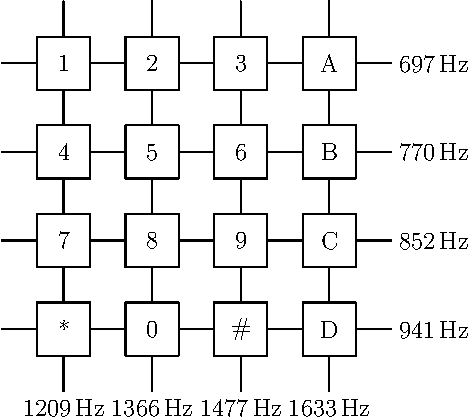
\includegraphics[height=.4\textheight]{pic/dtmf.pdf}
        \end{figure}
    \end{minipage}
\end{frame}

\begin{frame}[fragile]{\LaTeX{} Common Commands}
    \begin{exampleblock}{Commands}
        \centering
        \footnotesize
        \begin{tabular}{llll}
            \cmd{chapter} & \cmd{section} & \cmd{subsection} & \cmd{paragraph} \\
            Chapter & Section & Subsection & Paragraph \\\hline
            \cmd{centering} & \cmd{emph} & \cmd{verb} & \cmd{url} \\
            Centering & Emphasis & Verbatim & URL \\\hline
            \cmd{footnote} & \cmd{item} & \cmd{caption} & \cmd{includegraphics} \\
            Footnote & List Item & Caption & Include Graphics \\\hline
            \cmd{label} & \cmd{cite} & \cmd{ref} \\
            Label & Bibliography Citation & Cross Reference \\\hline
        \end{tabular}
    \end{exampleblock}
    \begin{exampleblock}{Environments}
        \centering
        \footnotesize
        \begin{tabular}{lll}
            \env{table} & \env{figure} & \env{equation}\\
            Table & Figure & Equation \\\hline
            \env{itemize} & \env{enumerate} & \env{description}\\
            Itemized List & Enumerated List & Description \\\hline
        \end{tabular}
    \end{exampleblock}
\end{frame}

\begin{frame}[fragile]{Example}
    \begin{minipage}{0.5\linewidth}
\begin{lstlisting}[language=TeX]
\begin{itemize}
  \item A \item B
  \item C
  \begin{itemize}
    \item C-1
  \end{itemize}
\end{itemize}
\end{lstlisting}
    \end{minipage}\hspace{1cm}
    \begin{minipage}{0.3\linewidth}
        \begin{itemize}
            \item A
            \item B
            \item C
            \begin{itemize}
                \item C-1
            \end{itemize}
        \end{itemize}
    \end{minipage}
    \medskip
    \pause
    \begin{minipage}{0.5\linewidth}
\begin{lstlisting}[language=TeX]
\begin{enumerate}
  \item Sun \item Moon
  \item Star
  \begin{itemize}
    \item[n+e] Star's...
  \end{itemize}
\end{enumerate}
\end{lstlisting}
    \end{minipage}\hspace{1cm}
    \begin{minipage}{0.3\linewidth}
        \begin{enumerate}
            \item Sun
            \item Moon
            \item Star
            \begin{itemize}
                \item[n+e] Star's...
            \end{itemize}
        \end{enumerate}
    \end{minipage}
\end{frame}

\begin{frame}[fragile]{\LaTeX{} math equations}
    \begin{columns}
        \begin{column}{.55\textwidth}
\begin{lstlisting}[language=TeX]
$V = \frac{4}{3}\pi r^3$

\[
  V = \frac{4}{3}\pi r^3
\]

\begin{equation}
  \label{eq:vsphere}
  V = \frac{4}{3}\pi r^3
\end{equation}
\end{lstlisting}
        \end{column}
        \begin{column}{.4\textwidth}
            $V = \frac{4}{3}\pi r^3$
            \[
                V = \frac{4}{3}\pi r^3
            \]
            \begin{equation}
                \label{eq:vsphere}
                V = \frac{4}{3}\pi r^3
            \end{equation}
        \end{column}
    \end{columns}
\end{frame}

\begin{frame}[fragile]
    \begin{columns}
        \column{.7\textwidth}
\begin{lstlisting}[language=TeX]
    \begin{table}[htbp]
      \caption{Number and Value}
      \label{tab:number}
      \centering
      \begin{tabular}{cl}
        \toprule
        Number & Value \\
        \midrule
        1 & 4.0 \\
        2 & 3.7 \\
        \bottomrule
      \end{tabular}
    \end{table}
    The number and meaning 
    of 
    Equation~(\ref{eq:vsphere}) 
    can be found in 
    Table~\ref{tab:number}.
\end{lstlisting}
        \column{.4\textwidth}
        \begin{table}[htpb]
            \centering
            \caption{Number and Value}
            \label{tab:number}
            \begin{tabular}{cl}\toprule
                Number & Value \\\midrule
                1 & 4.0\\
                2 & 3.7\\\bottomrule
            \end{tabular}
        \end{table}
        \normalsize The number and meaning of Equation~(\ref{eq:vsphere}) can be found in Table~\ref{tab:number}.
    \end{columns}
\end{frame}

\begin{frame}{Graphics}
    \begin{itemize}
        \item Vector graphics: eps, ps, pdf
        \begin{itemize}
            \item METAPOST, pstricks, pgf $\ldots$
            \item Xfig, Dia, Visio, Inkscape $\ldots$
            \item Save as pdf from Matlab / Excel, etc.
        \end{itemize}
        \item Raster graphics: png, jpg, tiff $\ldots$
        \begin{itemize}
            \item Improve clarity, avoid blurriness
            \item Should be avoided whenever possible
        \end{itemize}
    \end{itemize}
    \begin{figure}[htpb]
        \centering
        
\includegraphics[width=0.5\linewidth]{pic/BrandEvolution-NottinghamBlue.eps}
        \caption{This university logo is a vector graphic}
    \end{figure}
\end{frame}

\section{Results}
\begin{frame}
    The results show that
    \begin{itemize}
        \item ...
        \item ...
    \end{itemize}
\end{frame}

\section{References}

\begin{frame}[allowframebreaks]
    \bibliography{ref}
    \bibliographystyle{alpha}
    % If there are too many references, you can adjust the font size as follows:
    % \tiny\bibliographystyle{alpha}
\end{frame}

\begin{frame}
    \begin{center}
        {\Huge\calligra Thanks!}
    \end{center}
\end{frame}

\end{document}